\documentclass[12pt,letterpaper]{article}
\usepackage{graphicx,textcomp}
\usepackage{natbib}
\usepackage{setspace}
\usepackage{fullpage}
\usepackage{color}
\usepackage[reqno]{amsmath}
\usepackage{amsthm}
\usepackage{fancyvrb}
\usepackage{amssymb,enumerate}
\usepackage[all]{xy}
\usepackage{endnotes}
\usepackage{lscape}
\newtheorem{com}{Comment}
\usepackage{float}
\usepackage{hyperref}
\newtheorem{lem} {Lemma}
\newtheorem{prop}{Proposition}
\newtheorem{thm}{Theorem}
\newtheorem{defn}{Definition}
\newtheorem{cor}{Corollary}
\newtheorem{obs}{Observation}
\usepackage[compact]{titlesec}
\usepackage{dcolumn}
\usepackage{tikz}
\usetikzlibrary{arrows}
\usepackage{multirow}
\usepackage{xcolor}
\newcolumntype{.}{D{.}{.}{-1}}
\newcolumntype{d}[1]{D{.}{.}{#1}}
\definecolor{light-gray}{gray}{0.65}
\usepackage{url}
\usepackage{listings}
\usepackage{color}

\definecolor{codegreen}{rgb}{0,0.6,0}
\definecolor{codegray}{rgb}{0.5,0.5,0.5}
\definecolor{codepurple}{rgb}{0.58,0,0.82}
\definecolor{backcolour}{rgb}{0.95,0.95,0.92}

\lstdefinestyle{mystyle}{
	backgroundcolor=\color{backcolour},   
	commentstyle=\color{codegreen},
	keywordstyle=\color{magenta},
	numberstyle=\tiny\color{codegray},
	stringstyle=\color{codepurple},
	basicstyle=\footnotesize,
	breakatwhitespace=false,         
	breaklines=true,                 
	captionpos=b,                    
	keepspaces=true,                 
	numbers=left,                    
	numbersep=5pt,                  
	showspaces=false,                
	showstringspaces=false,
	showtabs=false,                  
	tabsize=2
}
\lstset{style=mystyle}
\newcommand{\Sref}[1]{Section~\ref{#1}}
\newtheorem{hyp}{Hypothesis}

% highlighting tools to identify final answer
\definecolor{pastelyellow}{RGB}{255, 250, 205}
\usepackage{soul}
\sethlcolor{pastelyellow}

\title{Problem Set 3}
\date{Due: November 12, 2026}
\author{Emily Zhang}


\begin{document}
	\maketitle
	\section*{Instructions}
	\begin{itemize}
		\item Please show your work! You may lose points by simply writing in the answer. If the problem requires you to execute commands in \texttt{R}, please include the code you used to get your answers. Please also include the \texttt{.R} file that contains your code. If you are not sure if work needs to be shown for a particular problem, please ask.
	\item Your homework should be submitted electronically on GitHub.
	\item This problem set is due before 23:59 on Thursday November 12, 2026. No late assignments will be accepted.

	\end{itemize}

		\vspace{.25cm}
	
\noindent In this problem set, you will run several regressions and create an add variable plot (see the lecture slides) in \texttt{R} using the \texttt{incumbents\_subset.csv} dataset. Include all of your code.

\vspace{0.5cm}
	
\section*{Question 1}
\vspace{.25cm}
\noindent We are interested in knowing how the difference in campaign spending between incumbent and challenger affects the incumbent's vote share. 
	\begin{enumerate}
		\item Run a regression where the outcome variable is \texttt{voteshare} and the explanatory variable is \texttt{difflog}.
		
		\lstinputlisting[language=R, firstline=52, lastline=56]{PS03_answersEZ.R}
		
% Table created by stargazer v.5.2.3 by Marek Hlavac, Social Policy Institute. E-mail: marek.hlavac at gmail.com
% Date and time: Thu, Nov 12, 2026 - 19:37:41
\begin{table}[H] \centering 
  \caption{Regression of voteshare on difflog} 
  \label{tab:q1} 
\begin{tabular}{@{\extracolsep{5pt}}lc} 
\\[-1.8ex]\hline 
\hline \\[-1.8ex] 
 & \multicolumn{1}{c}{\textit{Dependent variable:}} \\ 
\cline{2-2} 
\\[-1.8ex] & voteshare \\ 
\hline \\[-1.8ex] 
 difflog & 0.042$^{***}$ \\ 
  & (0.001) \\ 
  & \\ 
 Constant & 0.579$^{***}$ \\ 
  & (0.002) \\ 
  & \\ 
\hline \\[-1.8ex] 
Observations & 3,193 \\ 
R$^{2}$ & 0.367 \\ 
Adjusted R$^{2}$ & 0.367 \\ 
Residual Std. Error & 0.079 (df = 3191) \\ 
F Statistic & 1,852.791$^{***}$ (df = 1; 3191) \\ 
\hline 
\hline \\[-1.8ex] 
\textit{Note:}  & \multicolumn{1}{r}{$^{*}$p$<$0.1; $^{**}$p$<$0.05; $^{***}$p$<$0.01} \\ 
\end{tabular} 
\end{table}  

		
		\textbf{Analysis:}\\
		
		\item Make a scatterplot of the two variables and add the regression line. 
		
		\lstinputlisting[language=R, firstline=61, lastline=64]{PS03_answersEZ.R}
		\begin{figure}[H]\centering
			\caption{\footnotesize Incumbent vote share vs.\ difference in campaign spending (log).}
			\label{fig:q1}
			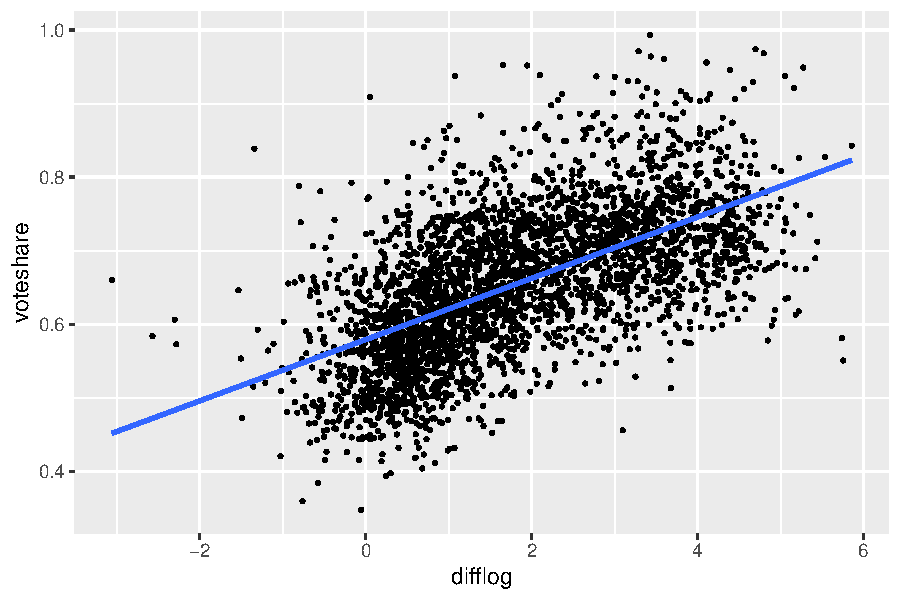
\includegraphics[width=.75\textwidth]{q1_plot.pdf}
		\end{figure}
		
		\textbf{Analysis:}\\
		
		\item Save the residuals of the model in a separate object.
		
		\lstinputlisting[language=R, firstline=68, lastline=69]{PS03_answersEZ.R}
		\begin{verbatim}
			Min.   1st Qu.    Median      Mean   3rd Qu.      Max. 
			-0.268319 -0.053454 -0.003769  0.000000  0.047798  0.327488 
		\end{verbatim}
		
		\textbf{Analysis:}\\
		
		\item Write the prediction equation.
		
		\lstinputlisting[language=R, linerange={73-74,77-78}]{PS03_answersEZ.R}
		\[ \widehat{\text{voteshare}} = 0.579 + 0.042 \times \text{difflog} \]
		
		\textbf{Analysis:}\\
	\end{enumerate}
	
\newpage

\section*{Question 2}
\noindent We are interested in knowing how the difference between incumbent and challenger's spending and the vote share of the presidential candidate of the incumbent's party are related.
	\begin{enumerate}
		\item Run a regression where the outcome variable is \texttt{presvote} and the explanatory variable is \texttt{difflog}.
		
		\lstinputlisting[language=R, firstline=86, lastline=90]{PS03_answersEZ.R}
		
% Table created by stargazer v.5.2.3 by Marek Hlavac, Social Policy Institute. E-mail: marek.hlavac at gmail.com
% Date and time: Thu, Nov 12, 2026 - 17:52:45
\begin{table}[H] \centering 
  \caption{Regression of presvote on difflog} 
  \label{tab:q2} 
\begin{tabular}{@{\extracolsep{5pt}}lc} 
\\[-1.8ex]\hline 
\hline \\[-1.8ex] 
 & \multicolumn{1}{c}{\textit{Dependent variable:}} \\ 
\cline{2-2} 
\\[-1.8ex] & presvote \\ 
\hline \\[-1.8ex] 
 difflog & 0.024$^{***}$ \\ 
  & (0.001) \\ 
  & \\ 
 Constant & 0.508$^{***}$ \\ 
  & (0.003) \\ 
  & \\ 
\hline \\[-1.8ex] 
Observations & 3,193 \\ 
R$^{2}$ & 0.088 \\ 
Adjusted R$^{2}$ & 0.088 \\ 
Residual Std. Error & 0.110 (df = 3191) \\ 
F Statistic & 307.715$^{***}$ (df = 1; 3191) \\ 
\hline 
\hline \\[-1.8ex] 
\textit{Note:}  & \multicolumn{1}{r}{$^{*}$p$<$0.1; $^{**}$p$<$0.05; $^{***}$p$<$0.01} \\ 
\end{tabular} 
\end{table}  

		
		\textbf{Analysis:}\\
		
		\item Make a scatterplot of the two variables and add the regression line. 
		
		\lstinputlisting[language=R, firstline=95, lastline=98]{PS03_answersEZ.R}
		\begin{figure}[H]\centering
			\caption{\footnotesize Presidential vote share vs.\ difference in campaign spending (log).}
			\label{fig:q2}
			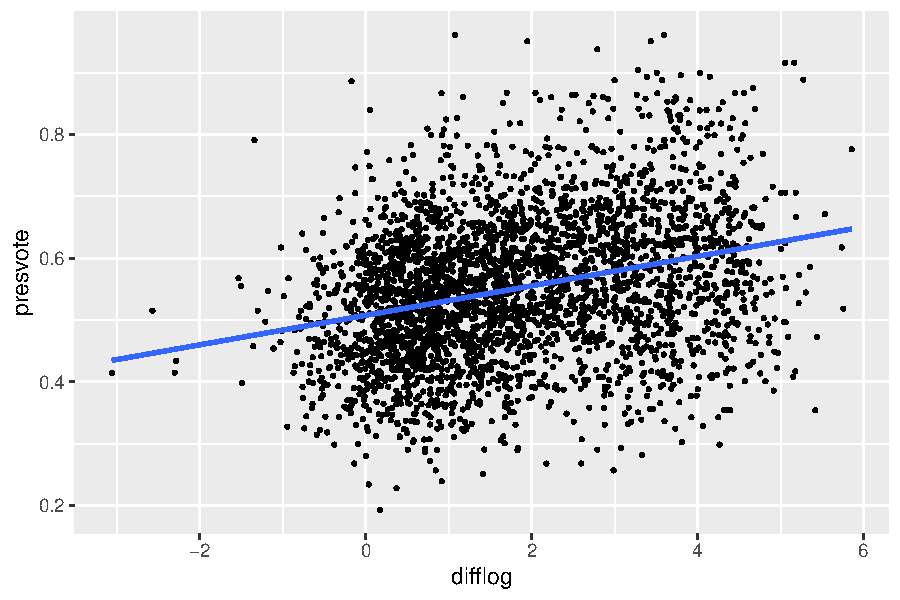
\includegraphics[width=.75\textwidth]{q2_plot.pdf}
		\end{figure}
		
		\textbf{Analysis:}\\
		
		\item Save the residuals of the model in a separate object.
		
		\lstinputlisting[language=R, firstline=102, lastline=103]{PS03_answersEZ.R}
		\begin{verbatim}
			Min.   1st Qu.    Median      Mean   3rd Qu.      Max. 
			-0.321965 -0.074069 -0.001018  0.000000  0.071507  0.427435 
		\end{verbatim}
		
		\textbf{Analysis:}\\
		
		\item Write the prediction equation.
		
		\lstinputlisting[language=R, linerange={107-108,111-112}]{PS03_answersEZ.R}
		\[ \widehat{\text{presvote}} = 0.508 + 0.024 \times \text{difflog} \]
		
		\textbf{Analysis:}\\
	\end{enumerate}
	
	\newpage	
\section*{Question 3}

\noindent We are interested in knowing how the vote share of the presidential candidate of the incumbent's party is associated with the incumbent's electoral success.
	\begin{enumerate}
		\item Run a regression where the outcome variable is \texttt{voteshare} and the explanatory variable is \texttt{presvote}.
		
		\lstinputlisting[language=R, firstline=119, lastline=123]{PS03_answersEZ.R}
		
% Table created by stargazer v.5.2.3 by Marek Hlavac, Social Policy Institute. E-mail: marek.hlavac at gmail.com
% Date and time: Thu, Nov 12, 2026 - 00:52:58
\begin{table}[!htbp] \centering 
  \caption{Regression of voteshare on presvote} 
  \label{tab:q3} 
\begin{tabular}{@{\extracolsep{5pt}}lc} 
\\[-1.8ex]\hline 
\hline \\[-1.8ex] 
 & \multicolumn{1}{c}{\textit{Dependent variable:}} \\ 
\cline{2-2} 
\\[-1.8ex] & voteshare \\ 
\hline \\[-1.8ex] 
 presvote & 0.388$^{***}$ \\ 
  & (0.013) \\ 
  & \\ 
 Constant & 0.441$^{***}$ \\ 
  & (0.008) \\ 
  & \\ 
\hline \\[-1.8ex] 
Observations & 3,193 \\ 
R$^{2}$ & 0.206 \\ 
Adjusted R$^{2}$ & 0.206 \\ 
Residual Std. Error & 0.088 (df = 3191) \\ 
F Statistic & 826.950$^{***}$ (df = 1; 3191) \\ 
\hline 
\hline \\[-1.8ex] 
\textit{Note:}  & \multicolumn{1}{r}{$^{*}$p$<$0.1; $^{**}$p$<$0.05; $^{***}$p$<$0.01} \\ 
\end{tabular} 
\end{table}  

		
		\textbf{Analysis:}\\
		
		\item Make a scatterplot of the two variables and add the regression line. 
		
		\lstinputlisting[language=R, firstline=128, lastline=131]{PS03_answersEZ.R}
		\begin{figure}[H]\centering
			\caption{\footnotesize Incumbent vote share vs.\ presidential vote share.}
			\label{fig:q3}
			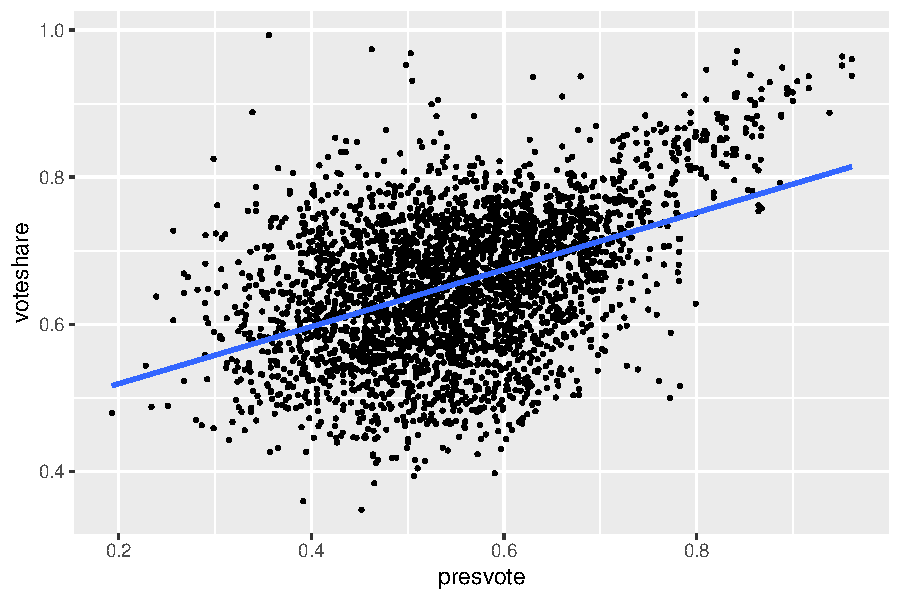
\includegraphics[width=.75\textwidth]{q3_plot.pdf}
		\end{figure}
		
		\textbf{Analysis:}\\
		
		\item Write the prediction equation.
		
		\lstinputlisting[language=R, linerange={135-136,139-140}]{PS03_answersEZ.R}
		\[ \widehat{\text{voteshare}} = 0.441 + 0.388 \times \text{presvote} \]
		
		\textbf{Analysis:}\\
	\end{enumerate}
	

\newpage	
\section*{Question 4}
\noindent The residuals from part (a) tell us how much of the variation in \texttt{voteshare} is $not$ explained by the difference in spending between incumbent and challenger. The residuals in part (b) tell us how much of the variation in \texttt{presvote} is $not$ explained by the difference in spending between incumbent and challenger in the district.
	\begin{enumerate}
		\item Run a regression where the outcome variable is the residuals from Question 1 and the explanatory variable is the residuals from Question 2.
		
		\lstinputlisting[language=R, linerange={148-148,151-155}]{PS03_answersEZ.R}
		
% Table created by stargazer v.5.2.3 by Marek Hlavac, Social Policy Institute. E-mail: marek.hlavac at gmail.com
% Date and time: Thu, Nov 12, 2026 - 00:53:00
\begin{table}[!htbp] \centering 
  \caption{Regression of Q1 residuals on Q2 residuals} 
  \label{tab:q4} 
\begin{tabular}{@{\extracolsep{5pt}}lc} 
\\[-1.8ex]\hline 
\hline \\[-1.8ex] 
 & \multicolumn{1}{c}{\textit{Dependent variable:}} \\ 
\cline{2-2} 
\\[-1.8ex] & residuals1 \\ 
\hline \\[-1.8ex] 
 residuals2 & 0.257$^{***}$ \\ 
  & (0.012) \\ 
  & \\ 
 Constant & $-$0.000 \\ 
  & (0.001) \\ 
  & \\ 
\hline \\[-1.8ex] 
Observations & 3,193 \\ 
R$^{2}$ & 0.130 \\ 
Adjusted R$^{2}$ & 0.130 \\ 
Residual Std. Error & 0.073 (df = 3191) \\ 
F Statistic & 476.975$^{***}$ (df = 1; 3191) \\ 
\hline 
\hline \\[-1.8ex] 
\textit{Note:}  & \multicolumn{1}{r}{$^{*}$p$<$0.1; $^{**}$p$<$0.05; $^{***}$p$<$0.01} \\ 
\end{tabular} 
\end{table}  

		
		\textbf{Analysis:}\\
		
		\item Make a scatterplot of the two residuals and add the regression line. 	
		
		\lstinputlisting[language=R, firstline=160, lastline=163]{PS03_answersEZ.R}
		\begin{figure}[H]\centering
			\caption{\footnotesize Added-variable plot: residuals of \texttt{voteshare} vs.\ residuals of \texttt{presvote} (both on \texttt{difflog}).}
			\label{fig:q4}
			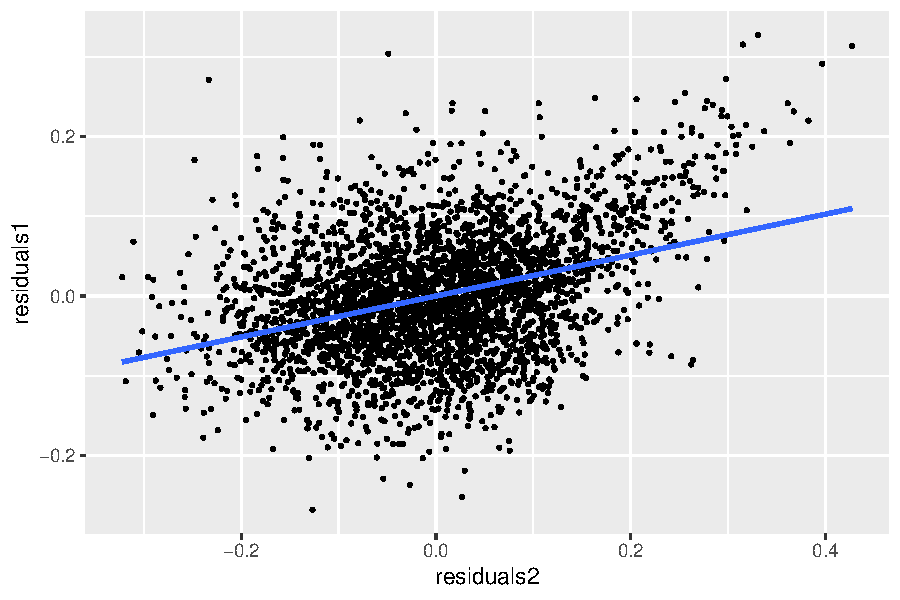
\includegraphics[width=.75\textwidth]{q4_plot.pdf}
		\end{figure}
		
		\textbf{Analysis:}\\
		
		\item Write the prediction equation.
		
		\lstinputlisting[language=R, linerange={167-168,171-172}]{PS03_answersEZ.R}
		\[ \widehat{\text{voteshare residual}} = 0 + 0.257 \times \text{presvote residual} \]
		
		\textbf{Analysis:}\\
	\end{enumerate}
	
	\newpage	

\section*{Question 5}
\noindent What if the incumbent's vote share is affected by both the president's popularity and the difference in spending between incumbent and challenger? 
	\begin{enumerate}
		\item Run a regression where the outcome variable is the incumbent's \texttt{voteshare} and the explanatory variables are \texttt{difflog} and \texttt{presvote}.	
		
		\lstinputlisting[language=R, firstline=180, lastline=184]{PS03_answersEZ.R}
		
% Table created by stargazer v.5.2.3 by Marek Hlavac, Social Policy Institute. E-mail: marek.hlavac at gmail.com
% Date and time: Thu, Nov 12, 2026 - 14:57:13
\begin{table}[H] \centering 
  \caption{Regression of voteshare on difflog and presvote} 
  \label{tab:q5} 
\begin{tabular}{@{\extracolsep{5pt}}lc} 
\\[-1.8ex]\hline 
\hline \\[-1.8ex] 
 & \multicolumn{1}{c}{\textit{Dependent variable:}} \\ 
\cline{2-2} 
\\[-1.8ex] & voteshare \\ 
\hline \\[-1.8ex] 
 difflog & 0.036$^{***}$ \\ 
  & (0.001) \\ 
  & \\ 
 presvote & 0.257$^{***}$ \\ 
  & (0.012) \\ 
  & \\ 
 Constant & 0.449$^{***}$ \\ 
  & (0.006) \\ 
  & \\ 
\hline \\[-1.8ex] 
Observations & 3,193 \\ 
R$^{2}$ & 0.450 \\ 
Adjusted R$^{2}$ & 0.449 \\ 
Residual Std. Error & 0.073 (df = 3190) \\ 
F Statistic & 1,302.947$^{***}$ (df = 2; 3190) \\ 
\hline 
\hline \\[-1.8ex] 
\textit{Note:}  & \multicolumn{1}{r}{$^{*}$p$<$0.1; $^{**}$p$<$0.05; $^{***}$p$<$0.01} \\ 
\end{tabular} 
\end{table}  

		
		\textbf{Analysis:}\\
		
		\item Write the prediction equation.
		
		\lstinputlisting[language=R, linerange={188-190,193-194}]{PS03_answersEZ.R}
		\[ \widehat{\text{voteshare}} = 0.449 + 0.036 \times \text{difflog} + 0.257 \times \text{presvote} \]
		
		\textbf{Analysis:}\\
		
		\item What is it in this output that is identical to the output in Question 4? Why do you think this is the case?
		
		\textbf{Analysis:}\\
	\end{enumerate}




\end{document}
